\chapter{Arhitectura soluţiei}

\section{Prezentare generală}
Alegria a fost conceputa ca o platforma de dezvoltare rapida, bazata pe modele. Prin folosirea unor metode de programare vizuala, cu blocuri refolosibile in mai multe aplicaţii diferite, utilizatorul poate sa îşi concentreze resursele asupra soluţiei finale, abstractizând detaliile implementării. 
Aplicaţia a fost construita pe baza unei arhitecturi modulare, cu module cat mai puţin cuplate, care sa permită modificări rapide si testarea modulelor individual. Urmărind aceasta gândire modulare, au fost s-au identificat 4 componente esenţiale: 
\begin{itemize}
	\item \textbf{Baza de date} Asigură stocarea datelor, dar si a entităţilor existente in aplicaţie;
	\item \textbf{Interfaţa web pentru management} O interfaţă uşor de utilizat care sa permită  utilizatorului să manipuleze canale, diagrame, blocuri de procesare, dar si alţi utilizatori
	\item \textbf{API-ul pentru date} Un API specializat pentru adăugare de date, achiziţionarea datelor, dar si sa permită altor dispozitive sa fie notificate de fiecare data când apar date noi.
	\item \textbf{Elemente de procesare} Asigură procesarea datelor, atât in cadrul blocurilor de procesare, dar si in cadrul diagramelor funcţionale.
\end{itemize}
\begin{figure}
	\centering
	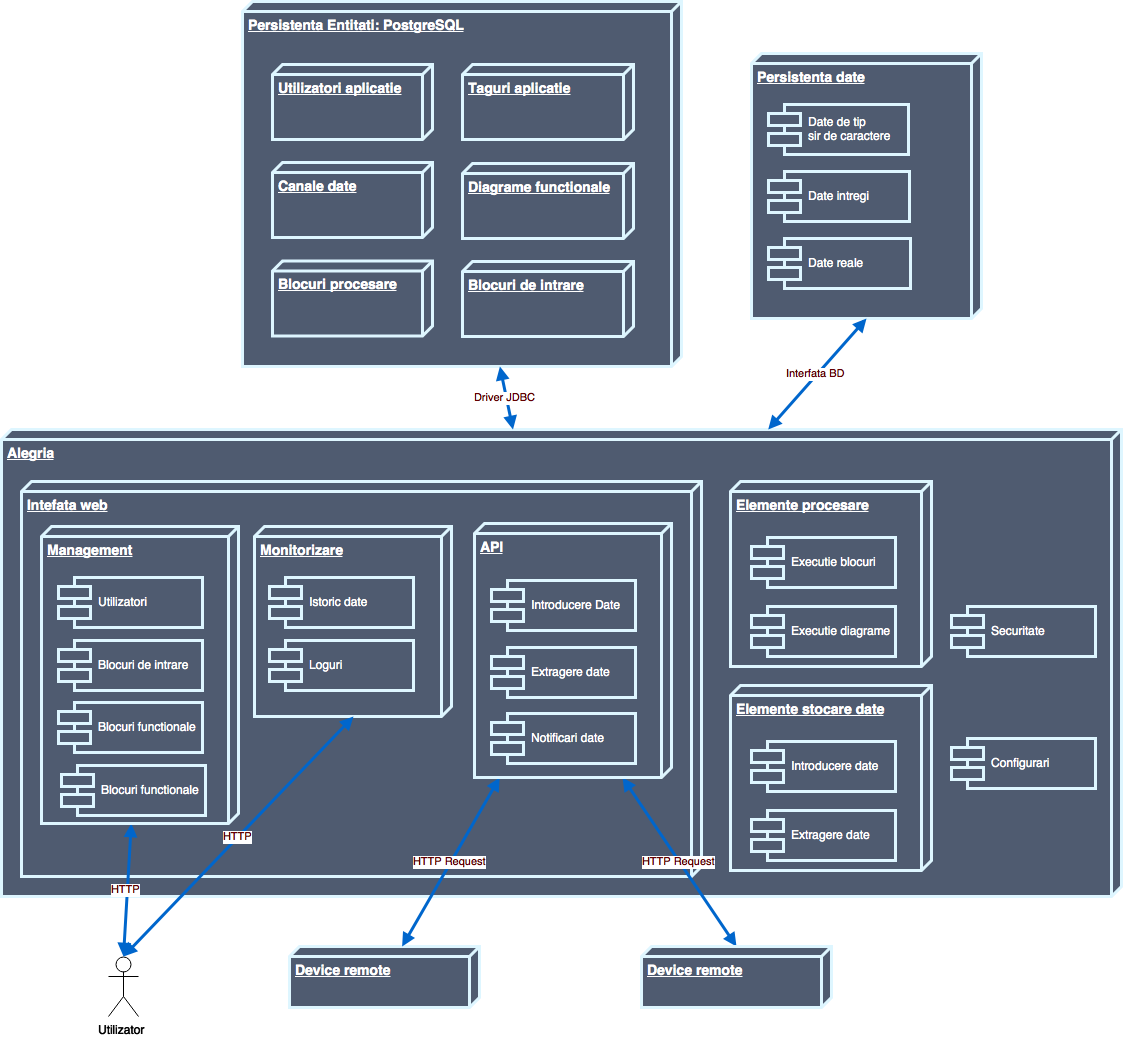
\includegraphics[width=1.3\textwidth, center]{arhitecturaGenerala}
	\caption{Arhitectura generala a aplicaţiei}
	\label{fig:arhitecture}
\end{figure}

In vederea implementării sistemului s-au identificat următoarele elemente componente esenţiale, componente ce reprezinta elementele constructive a sistemului. Acestea, au reprezentare atât in baza de date, ca entităţi, cat si in aplicaţia Java, ca clase. Identificarea acestor elemente s-a făcut pe baza analizei cazurilor de utilizare a produsului, in care s-au investigat metodele prin actorii interacţionează cu sistemul.
\begin{itemize}
\label{list:entities}
\item \textbf{Canalul de date:} reprezinta elementul de baza a sistemului, care asigura recepţia, persistenta si emiterea de date. Datele dintr-un canal trebuie sa respecte un format prestabilit la crearea canalului. Pentru transformarea datelor in formatul stabilit, se poate introduce un bloc de pre-procesarea care transforma datele din un format brut in formatul standard.
\item \textbf{Blocul de intrare:} elementul de mapează un element din lumea real in interiorul platformei. Blocurile de intrare permit gruparea mai multor canale de date într-o structura unica.
\item \textbf{Blocul de procesare:} elementul dinamic al aplicaţiei, ce aplica transformări asupra datelor. Un bloc de procesare primeşte ca intrări mai multe canale de date, si are la ieşire un alt canal de date. Utilizatorul poate folosi blocuri standard, existente in sistem, sau poate implementa blocuri noi direct in interfaţa programului.
\item \textbf{Diagrama funcţie bloc(FBD):}  foloseşte blocuri de intrare, canale de date si blocuri de procesare pentru a descrie o funcţie complexa intre intrări si o ieşire. Aceste diagrame folosesc la date aflate pe canale de date, care sunt trimise către blocuri de procesare si, la final se obţine un singur rezultat care este salvat pe un canal de date.
\end{itemize}

\subsection{Baza de date}

Fiind vorba despre o aplicaţie puternic bazata pe date, aceasta are nevoie de un nivel de persistenta de înaltă performaţă. 
Urmărind arhitectura propusă din \cref{fig:arhitecture}, putem identifica doua cazuri de utilizare pentru baza de date: 
\begin{itemize}
	\item Stocarea modelului entităţilor: fiecare entitate descrisa in lista de mai sus trebuie stocata in baza de date într-o structura relaţională. Entităţile sunt puternic interconectate, iar o baza de date relaţională, de tip SQL este recomandata in acest caz. 
	Din punct de vedere a dimensiunii setului de date, chiar si in aplicaţiile de mare complexitate, este vorba despre doar câteva milioane de înregistrări, factorul care face acest număr să crească fiind conectarea a tot mai mult dispozitive, ce duce la din ce in ce mai multe canale de date. Astfel, stocarea entităţilor nu va aduce probleme de performaţă. 
	\item Stocarea datelor: in baza de date vor fi stocate atât datele primite pe fiecare canal asociat unui bloc de intrare, cat si datele procesate de diagrame. Aceste date au un puternic caracter istoric, reprezentând o serie de timp, in care se retine, pentru fiecare punct de date, valoarea la un anumit moment. Problema stocării acestor date este una mai complicata, datorita necesităţii unei puternice scalari a bazei de date. Această problemă reprezinta un caz de utilizare pentru o baza de date NoSQL, sau chiar o baza de date specializata in stocarea seriilor de timp \autocite{openTSDB}.  
\end{itemize}

\subsection{Aplicaţia Java}
Legătura dintre baza de date si utilizatorii finali se face prin intermediul unei aplicaţii Java complexe, care este obiectul acestui proiect. Aplicaţia conţine toată logica platformei, de la operaţii asupra entităţilor din baza de date, la adăugarea, si extragerea datelor, cat si pentru procesarea datelor. 
Separarea modulelor s-a făcut pe baza scopului acestora:
\begin{itemize}
	\item \textbf{Administrare}: pentru administrarea entităţilor din baza de date. Aceste module permit operaţii de căutare si afişare, dar si de creere, editare si ştergere a utilizatorilor, a blocurilor de intrare si funcţionale precum si a diagramelor. Fiecare dispune de o interfaţă HTML5 in care moderna. 
	\item \textbf{Monitorizare}: permit monitorizarea execuţiei aplicaţiei, de la vizualizat loguri pentru a diagnostica probleme, la realizarea de grafice a datelor pe anumite canale. Tot aici este disponibila si funcţia de a exporta date in formate uzuale, ca CSV sau fişiere Microsoft Excel.
	\item \textbf{API}: aplicaţia dispune si de un API pentru a fi folosita programatic de către alte aplicaţii externe. Acesta poate fi considerat ca fiind format din doua componente: serviciile pentru administrarea entităţilor, si cele pentru adăugarea si extragerea datelor.
	\item \textbf{Elemente de procesare}: împărţite in doua subcategorii: cele pentru procesarea blocurilor de intrare si de procesare, si cele pentru procesarea diagramelor.
	\item \textbf{Elemente stocare date}: permit interfaţarea cu sursele de date. Acestea asigura servicii de introducere si extragere a datelor, printr-o interfaţă abstracta, care nu tine cont de modul in care baza de date este implementata.
	\item \textbf{Alte module}: asigura, printre altele securitatea aplicaţiei.
\end{itemize}

\section{Entităţi}
\subsection{Punctul de date}

Punctul de date reprezinta elementul constructiv al sistemul, care este obiectul procesării, stocării si distribuţiei este punctul de date. 
Sistemul accepta intern date in formatele: 
\begin{wrapfigure}{r}{0.38\textwidth}
	\centering
	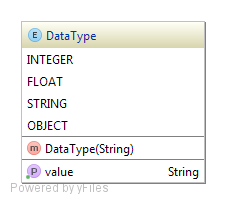
\includegraphics[width=0.38\textwidth]{dataType}
	\caption{Tipurile de date acceptate in sistem}
\end{wrapfigure}
\begin{itemize}
	\item \textbf{Întreg}: numere de la $-2^{63}$ la $2^{63} -1$, fără virgula, foloseşte \textit{Long} pentru reprezentare interna;
	\item \textbf{Real}: numere cu virgula, având dubla precizie, reprezentate cu 64-bit conform standardului \autocite{4610935} IEEE 754  foloseşte \textit{Double} pentru reprezentare interna;
	\item \textbf{Sir de caractere}: Un sir de fără limite a lungimii, care trebuie formatat conform \autocite{rfc4627}. 
	\item \textbf{Obiect}: Un obiect Java serializat in text. Intern, asemănător cu tipul de date String. 
\end{itemize}

\begin{figure}[h]
	\centering
	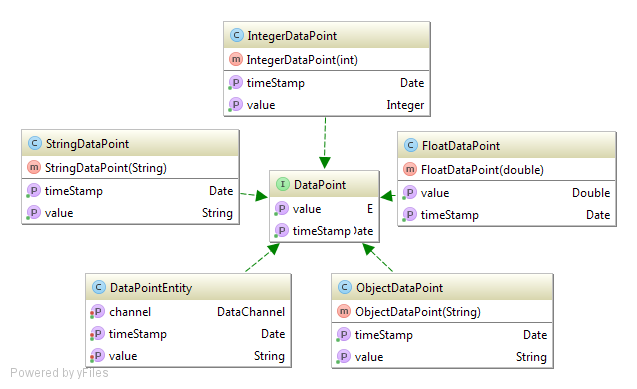
\includegraphics[width=1.1\textwidth, center]{dataPoint}
	\caption{Clasele care implementează interfaţa DataPoint}
\end{figure}

\subsection{Canalul de date}

Canalul de date este entitatea care asigura "curgerea" datelor prin sistem. Orice punct de date din sistem aparţine unui canal, acest lucru fiind realizat drept constrângere atât la nivelul aplicaţiei, cat si la nivelul bazei de date.
\begin{figure}[h]
	\centering
	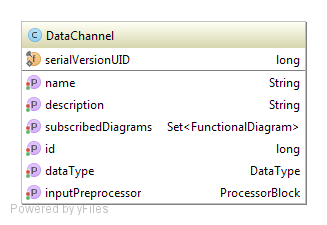
\includegraphics[width=0.55\textwidth]{dataChannel}
	\caption{Clasa DataChannel}
\end{figure}

Canalul este si mijlocul prin care utilizatorul interacţionează cu punctele de date. Când un dispozitiv adaugă date noi in sistem, acestea sunt ataşate unui canal, care poate fi folosit ca una dintre intrările unei diagrame de blocuri funcţionale. De asemenea, datele procesate de o diagrama sunt ataşate unui canal, permiţând apoi accesul pentru extragerea de datelor deja existente, si pentru a primi notificări de fiecare data când pe un canal apar informaţii noi.

Un canal mai poate avea si un bloc de preprocesare ataşat. Acesta este executat de fiecare data când date noi încearcă sa fie introduse in canal, permiţând validarea si transformarea datelor brute in date ce respecta tipul de date al canalului.  
\subsection{Blocul de intrare}
Blocurile de intrare modelează elemente reale in Alegria, grupând mai multe canale de date si expunându-le pentru a permite introducerea de date din exterior. Acestea descriu modul in care datele sunt legate de un element real. 

Spre exemplu, o sursă de alimentare neîntreruptibilă care este inteligenta si conectata din \cref{fig:ups} poate fi privită ca un bloc de intrare, iar fiecare senzor de pe aceasta fiind canal de date. Dispozitivul inteligent devine astfel conectat la platforma si acesta poate sa trimită date către aceasta. Pentru ca datele pot sa aibă perioade de eşantionare diferite, dispozitivul trimite date către unul sau mai multe canale, fără sa fie forţat sa trimită date pentru toate canalele odată.

Un alt mod in care blocurile de intrare pot fi privite este ca obiecte, sau "Things" in cadrul Internetului Tuturor Lucrurilor (IoT). Astfel, putem privi blocurile de intrare ca dispozitive ce monitorizează bătăile inimii sau activitatea celebrară, ca automobile cu reţele complexe de senzori, sau chiar aplicaţii business ce generează date in timp real. Prin acest mijloc, dispozitive inteligente se pot conecta in platforma, fie trimiţând direct date, fie prin intermediul unui agent care se afla pe dispozitiv, agent ce funcţionează ca un gateway.

\begin{figure}[H]
	\centering
	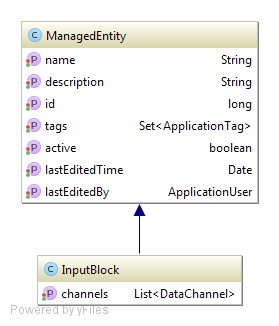
\includegraphics[width=0.55\textwidth]{inputBlock}
	\caption{Clasa InputBlock}
\end{figure}
\begin{figure}[H]
	\centering
	\includegraphics[width=\textwidth]{UPS}
	\caption{Modelarea unui UPS inteligent in Alegria}
	\label{fig:ups}
\end{figure}

\subsection{Blocul de procesare}

Blocurile de procesare realizează operaţiile transformare a datelor. Din punct de vedere funcţional, acestea au la intrare ultimele date introduse de pe mai multe canale si returnează un singur punct de date, comportându-se ca un element de tip "back-box"\autocite{functionBlocks}. Pentru implementare, utilizatorul foloseşte limbaje dinamice moderne, ca JavaScript sau Ruby, scriind funcţiile direct in interfaţa web. Aceste funcţii sunt rulate de către server. 
Conceptul de blocuri de procesare reprezinta o implementare a blocurilor de operaţii definite in standardul \autocite[Apendix C]{IEC61131-3}.

Blocuri pre-implementate exista in orice instanta a platformei care permit rezolvarea de probleme complexe cu cunoştinţe minime de programare.
Un alt aspect important al blocurilor de procesare, este ca ele sunt complet independente, ele oferind doar mijloace de prelucrare a unor date abstracte. Aceasta abstractizare permite refolosirea lor in mai multe proiecte. Spre exemplu, un bloc care face media tuturor intrărilor nu tine cont de originea datelor. 

Blocurile \textbf{nu au memorie statica}. Ele pot folosi informaţii exterioare, cum ar fi timpul curent al zilei, sau alte informaţii din sistem, însa ele nu au stare interioara. Astfel, se poate considera ca blocurile reprezinta un element combinaţional, si nu unul secvenţial.
\begin{figure}[H]
	\centering
	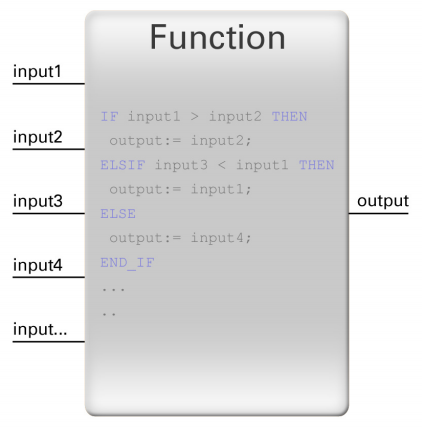
\includegraphics[width=0.6\textwidth]{exempluBlock}
	\caption{Exemplu bloc de procesare}
\end{figure}

\begin{figure}[H]
	\centering
	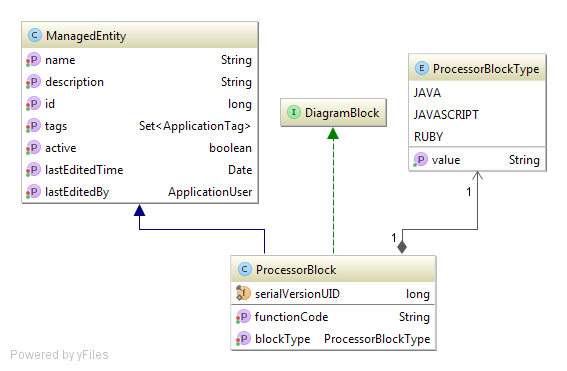
\includegraphics[width=\textwidth]{processorBlock}
	\caption{Clasa ProcessorBlock}
\end{figure}

\subsection{Diagrama funcţie bloc(FBD)}

Diagramele funcţie bloc reprezinta o implementare a unuia din cele patru limbare de programare pentru automate programabile, specificate de standardul IEC 61131-3:2013 \autocite[128-140]{IEC61131-3}. FBD-ul este un limbaj de control al procesului, in mod normal, toate blocurile de procesare dintr-o diagrama fiind executate.
In cel mai simplu caz de utilizare, un FBD realizează următoarele operaţii:
\begin{itemize}
	\item Accepta date de intrare de la unul sau mai multe canale;
	\item Realizează o operaţie de transformare asupra acelor date folosind un bloc de procesare;
	\item Salvează rezultatul pe un canal de ieşire.
\end{itemize}
Legăturile dintre blocurile de procesare sunt unidirecţionale. Un bloc de procesare poate trimite rezultatul al unul sau mai multe blocuri, iar o intrare poate fi conectata la o singura ieşire. Transmiterea de date se face fără întârzieri. Diagramele sunt executate in ordinea definita de ordonarea topologica a nodurilor din graful ce defineşte diagrama \autocite[20-50]{IEC61499}. 
\begin{figure}[H]
	\centering
	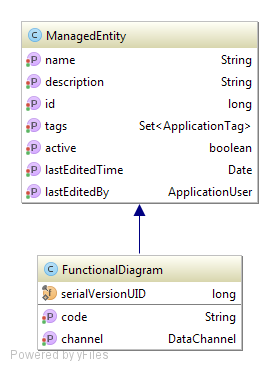
\includegraphics[width=0.5\textwidth]{functionalDiagram}
	\caption{Clasa FunctionalDiagram}
\end{figure}

\begin{figure}[H]
	\centering
	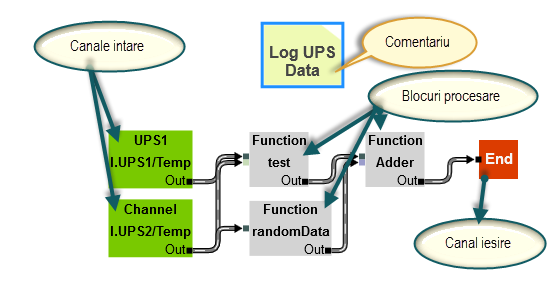
\includegraphics[width=0.95\textwidth]{exempluDiagrama}
	\caption{Exemplu diagrama funcţională}
	\label{fig:exempluDiagrama}
\end{figure}

\section{Primirea datelor}
Primirea datelor se face prin intermediul unei interfeţe de transfer a stării (REST). Mai multe formate sunt incluse pentru integrarea mai uşoară cu sisteme deja existente. Astfel, au fost implementate mai multe procesoare care primesc date atât într-un format special, cat si in formate standard in industrie.
Astfel, doua modalităţi de trimitere a datelor exista in sistem:
\begin{itemize}
	\item Trimitere către un singur canal, un singur punct odată: pe baza serviciului\\ \textit{/api/put/{inputId}/{channelId}/{data}}. Acest serviciu adaugă un singur punct in baza de date, la momentul curent. Folosit pentru sisteme care trimit date rar, si nu trebuie sa se tina cont de data locala de pe device-ul care a trimis punctul de date.
	\item In formatul standard folosit de openTDSB in care au fost introduse următoarele modificări care păstrează totuşi compatibilitatea: metricile reprezinta numele canalului, iar tag-urile sunt opţionale. Se acceptat atât formatul in care într-o cerere se afla un singur punct, cat si formatul cu o lista de puncte. Canalele dintr-o cere multidimensionala nu trebuie sa facă parte din acelaşi bloc de intrare. Acest mod de introducere a datelor este sugerat pentru sistemele care folosesc mai multe canale de date si care trimit seturi de date mai mari printr-o singura cerere. Spre exemplu, un dispozitiv poate trimite date de pe mai multi senzori, si poate stoca local mai multe măsurători pe acelaşi senzor pentru a trimite toate datele odată.
\end{itemize}
Odată primite, noile puncte de date trec prin procesul descris in \cref{fig:intrareDate}:
\begin{enumerate}
	\item Se interoghează baza de date pentru detalii privind canalul ce tocmai a primit date.
	\item Dacă un preprocesor exista pe canalul specificat, atunci el este încărcat.
	\item Se executa preprocesorul cu punctul de date primit
	\item Se salvează rezultatul in baza de date.
	\item Asincron, se lansează toate diagramele care trebuie sa se execute atunci când se primesc date noi pe acest canal.
	\item Asincron, se informează ascultătorii ca canalul a primit date noi.
\end{enumerate}
\begin{landscape}
	\begin{figure}
		\centering
		\includegraphics[width=1.7\textwidth]{introducereDate}
		\caption{Diagrama de secvente pentru introducerea de noi date si execuţia diagramelor}
		\label{fig:intrareDate}
	\end{figure}
\end{landscape}

\section{Executarea unei diagrame} 
\Cref{fig:intrareDate} prezintă si modul in care o diagrama este executată. Diagramele sunt lansate in execuţie de fiecare dată când un canal folosit in ea primeşte informaţii noi. Dacă doua canale primesc date în acelaşi timp, atunci diagrama va fi lansata in execuţie tot de doua ori, pentru ambele puncte de date primite.

\subsection{Ordinea execuţiei blocurilor}
Problema ordinii execuţiei unei FBD este intens dezbătută atât in literatura, cat si în aplicaţiile industriale. Cum standardul \textit{IEC61131-3} \autocite{IEC61131-3} nu propune o soluţie pentru ordinea de execuţie, producătorii industriali folosesc metode proprii, de la separarea blocurilor într-un tabel si executarea de la stânga la dreapta, sus in jos \autocite[11]{TM241}, la definirea manuala a ordinii execuţiei \autocite[11]{Logix5000} sau folosind algoritmi care determina automat ordinea de execuţie \autocite[5]{GEFANUC}.

In implementarea din Alegria s-a ales proiectarea unei metode automate pentru depistarea ordinii in care diagrama trebuie executata. Deoarece o diagrama reprezinta un graf aciclic orientat, prima etapa a execuţiei este transformarea într-un graf reprezentat prin lista de adiacenta, unde fiecare bloc de intrare, bloc si de procesare reprezinta un nod. Din aceasta reprezentare se omit blocurile de comentarii. Odată ce transformarea a fost efectuata cu succes se încerca aplicarea unui algoritm de sortare topologica\autocite{toposort} a grafului obţinut. Aceasta sortare implica găsirea unei ordini astfel încât pentru orice arc orientat $uv$ de la  $u$ la $v$, $u$ este înaintea lui $v$. 
Matematic problema poate fi formulata astfel:

\begin{definition} 
O \textbf{ordine topologica}, notata $ord_D$, au unui graf orientat aciclic $D = (V,E)$ atribuie fiecărui nod o valoare astfel încât $ord_D(x) < ord_D(y)$ pentru orice arc $ x \rightarrow y \in E$.
\end{definition}
Mai multi algoritmi pentru efectuarea unei asemenea sortări exista in literatura \autocite{toposortArticle}, însa, deoarece grafurile in discuţie sunt statice, la care nu se adaugă sau se şterg noduri, s-a ales un algoritm clasic, stabil din punct de vedere numeric descris de Kahn in 1962 \autocite{topoKahn}.

Simplificat, algoritmul implementat urmăreşte următorii paşi:
\begin{enumerate}
	\item Identifica toate nodurile spre care nu vine nici un arc. Valoarea acestor noduri va fi $0$. In cazul diagramelor, este vorba de toate canalele de intrare, si de blocurile de procesare care nu au nici o intrare. Dacă aceste noduri nu exista, înseamnă ca graful nu respecta condiţia de graf aciclic, deci acesta nu va putea fi executat.
	\item Se alege unul din din nodurile găsite mai sus.
	\item Se şterge acest nod de valoare unu, împreună cu toate arcele care ies din el.
	\item Se repeta paşii 1 si 2 pana când nu mai exista noduri in graf.
\end{enumerate}
Algoritmul descris mai sus rulează in $\mathcal{O}(V + E)$. 

\begin{algorithm}[H]
	\KwData{Un graf orientat acliclic reprezentat prin lista de adiacenta}
	\KwResult{Lista nodurilor ordonate topologic}
	$L \gets$ Lista goala ce va conţine nodurile sortate \;
	$S \gets$ Lista tuturor nodurilor spre care nu exista nici un arc \;
	\While{ $S$ conţine elemente }{ 
		şterge nodul $n$ din $S$ \;
		introdu nodul $n$ in $L$ \;
		\ForEach{nod $m$ care are un arc $e$ de la $n$ la $m$}{
			şterge arcul $e$ din graf\;
			\If{$m$ nu mai are arce spre el}
			{inserează $m$ in $S$}
		}{
	} 
	
}
	\eIf{mai exista arce in graf}
	{\Return{\textbf{Eroare:} Graful are cel puţin un ciclu}}{
	{\Return{$L$ (graful sortat topologic)}}
}
\label{alg:khan}
\caption{Algoritmul lui Khan pentru sortare topologica}
\end{algorithm}

Astfel, pentru diagrama din \cref{fig:exempluDiagrama}, o posibila ordine de execuţie este descrisa in \cref{fig:executionOrder}.
\begin{figure}[H]
	\centering
	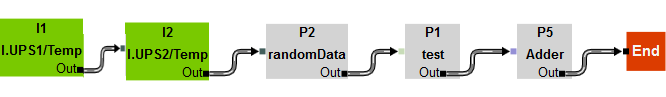
\includegraphics[width=\textwidth]{diagramExecutionOrder}
	\caption{Ordinea execuţiei pentru diagrama din \cref{fig:exempluDiagrama}}
	\label{fig:executionOrder}
\end{figure}
După cum se observa si in \cref{alg:khan} acesta poate detecta grafuri care conţin cicluri si nu pot fi rezolvate. Aceasta verificare permite detectarea cazurilor, precum cel din diagrama \ref{fig:badDiagram}, si permite informarea utilizatorului pentru ca acesta sa rezolve problema.
\begin{figure}[H]
	\centering
	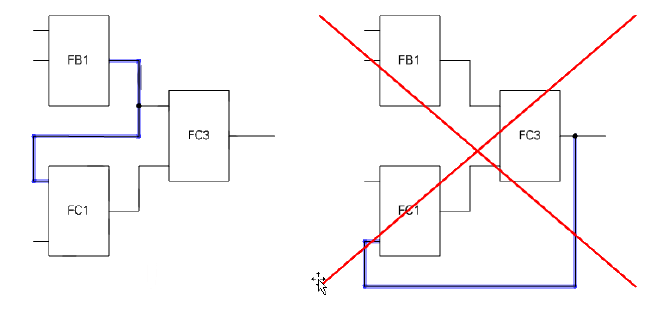
\includegraphics[width=0.95\textwidth]{badDiagram}
	\caption{Diagrama ce conţine cicluri}
	\label{fig:badDiagram}
\end{figure}

Deşi ciclurile la nivel de diagrama nu sunt permise, cele la nivel de canal sunt. Astfel, ieşirea unei diagrame poate fi setata ca intrare pentru aceeaşi diagrama, permiţând executarea într-o bucla, deoarece odată ce o diagrama se termina de executat si salvează rezultatul pe canal, aceasta se relansează in execuţie cu noua informaţie. Cu astfel de bucle se poate implementa diagrame ce interacţionează intre ele. Un alt aspect pozitiv al faptului ca intrările unor diagrame pot fi ieşirile unor alte diagrame este faptul ca procese foarte complexe pot fi descompuse in părţile componente prin simpla înlănţuire a diagramelor.

\subsection{Generarea rezultatului}
Odată ce ordinea de execuţie a fost calculată, procesul de calcul al rezultatului este destul de simplu:

\begin{algorithm}[H]
	\KwData{Lista nodurilor ordonate topologic}
	\KwResult{Punctul de date ce trebuie adaugat pe canalul de iesire a diagramei}
	$rezultate \gets$ Relaţie cheie-valoare intre nod si rezultatul execuţiei lui\;
	$L \gets$ Lista ce conţine nodurile sortate \;
	\ForEach{nod $m$ din $L$}{
		$intrari \gets$ Lista goala de intrări pentru nodul $m$ \;
		\ForEach{arc de la $n$ către $m$}{
			\eIf{In $rezultate$ exista rezultatul pentru blocul $n$}
			{Adaugă in $intrari$ valoarea de la $rezultate(n)$\;}{
				{\Return{\textbf{Eroare:} Graful nu poate fi executat\;}}
			}	
		}
			\eIf{$m$ este un bloc de procesare}
			{Executa blocul folosind intrările $intrari$\;
				Adaugă in $rezultate$ valoarea calculata\;}{
				\ElseIf{$m$ este un canal de date} {
						Adaugă in $rezultate$ ultima valoare de pe canal\;}
			} 
	}

{\Return{Ultima valoare din $rezultate$}}
\label{alg:executeDiagram}
\caption{Execuţia unei diagrame FBD}
\end{algorithm}

